\documentclass[12pt,a4paper]{article}

\usepackage[a4paper,margin=1in]{geometry}
\usepackage{graphicx}
\usepackage{amsmath}
\usepackage{booktabs}
\usepackage{hyperref}
\usepackage{setspace}

\setstretch{1.2}
\hypersetup{colorlinks=true, linkcolor=black, urlcolor=blue}

\title{\textbf{IntelliCharge360\\
Intelligent EV Charging Demand Prediction\\
\large  From Usage Analytics to Infrastructure Planning}}

\author{Presented By:-
Rashmi Anand(2401010374)\\
Samiksha Jangid(2401010410)\\
Shubhaang Kataruka (2401010450)\\
Ankit Raj Singh(2401010075)}
\date{}

\begin{document}


\maketitle



\begin{abstract}
The rapid adoption of electric vehicles (EVs) has introduced dynamic demand patterns in charging infrastructure. 
Unpredictable load surges can lead to congestion, inefficient infrastructure planning, and grid instability. 
This project presents a machine learning-driven system for predicting hourly EV charging demand using real-world charging session data. 
The system integrates structured preprocessing, time-series feature engineering, regression modeling, evaluation using MAE, RMSE, and R\textsuperscript{2}, and deployment via an interactive Streamlit dashboard. 
The architecture is modular and scalable, enabling future extension into agentic infrastructure planning and autonomous grid optimization.
\end{abstract}



\section{Problem Statement}

With increasing EV adoption, charging stations experience fluctuating demand based on time-of-day, location, and usage patterns. 
Infrastructure planners require predictive systems to:

\begin{itemize}
    \item Forecast hourly charging demand
    \item Identify congestion risk
    \item Optimize charger placement
    \item Improve grid-level planning decisions
\end{itemize}

The objective of this project is to develop a robust machine learning model that predicts EV charging demand using historical session-level data.

\section{Data Description}

The dataset was provided in JSON format containing charging session records with the following fields:

\begin{itemize}
    \item connectionTime
    \item disconnectTime
    \item kWhDelivered
    \item stationID
\end{itemize}

\subsection{JSON to CSV Conversion}

The raw JSON data was converted into CSV format for structured preprocessing:

\begin{verbatim}
df = pd.DataFrame(data["_items"])
df.to_csv("raw_dataset.csv", index=False)
\end{verbatim}

This enabled standardized tabular analysis using Pandas and Scikit-Learn.

\section{Exploratory Data Analysis}

EDA revealed:

\begin{itemize}
    \item Missing timestamps
    \item Invalid session durations
    \item Skewed energy distribution
    \item Strong hourly seasonality
    \item Evening demand peaks
    \item Station-wise variation
\end{itemize}

These findings guided feature engineering and model selection.

\section{Data Preprocessing}

The following cleaning steps were applied:

\begin{itemize}
    \item Removed null values in critical columns
    \item Parsed timestamps safely
    \item Removed invalid sessions
    \item Removed zero or negative energy values
    \item Applied IQR-based outlier handling
\end{itemize}

Session-level data was aggregated into hourly station-level demand to create structured time-series data.

\section{Feature Engineering}

The following features were engineered:

\begin{itemize}
    \item Hour of Day
    \item Day of Week
    \item Month
    \item Week of Year
    \item Cyclical encoding (sin/cos)
    \item Lag-1 demand
    \item Rolling 3-hour mean
    \item Rolling 24-hour mean
    \item Station encoding
\end{itemize}

Lag features were created before splitting to avoid data leakage.

\section{Methodology}

A chronological 80-20 train-test split was used.

Models evaluated:

\begin{itemize}
    \item Linear Regression
    \item Random Forest (200 trees)
    \item Gradient Boosting
    \item LightGBM
\end{itemize}

Tree-based models were chosen due to their ability to capture nonlinear demand patterns in structured data.

\section{Evaluation}

Models were evaluated using:

\begin{itemize}
    \item Mean Absolute Error (MAE)
    \item Root Mean Squared Error (RMSE)
    \item R\textsuperscript{2} Score
\section{Rationale Behind Model and Metric Selection}

\subsection{Why These Models Were Chosen}

The EV charging demand prediction task is a structured tabular regression problem with nonlinear temporal patterns. 
Therefore, multiple regression models with increasing complexity were evaluated to ensure robustness and performance comparison.

\textbf{1. Linear Regression (Baseline)}

Linear Regression was implemented as a baseline model to establish a minimum performance benchmark. 
It provides interpretability and helps assess whether demand patterns are linearly separable using engineered temporal features.

\textbf{2. Random Forest Regressor}

Random Forest was selected because:

\begin{itemize}
    \item It captures nonlinear feature interactions.
    \item It is robust to noise and outliers.
    \item It provides intrinsic feature importance scores.
    \item It performs well on structured tabular datasets.
\end{itemize}

\textbf{3. Gradient Boosting Regressor}

Gradient Boosting was used to:

\begin{itemize}
    \item Reduce bias through sequential learning.
    \item Capture complex demand patterns.
    \item Improve predictive accuracy over bagging-based methods.
\end{itemize}

\textbf{4. LightGBM Regressor}

LightGBM was selected due to:

\begin{itemize}
    \item Histogram-based fast training.
    \item Efficient handling of large datasets.
    \item Strong performance on time-dependent structured data.
    \item Better scalability for future deployment.
\end{itemize}

Tree-based ensemble methods are particularly effective for tabular data where feature interactions and nonlinearities exist, which is characteristic of EV charging demand.

\subsection{Why These Evaluation Metrics Were Used}

The task is a regression problem; therefore, regression-based evaluation metrics were selected.

\textbf{Mean Absolute Error (MAE):}

\begin{itemize}
    \item Measures average magnitude of prediction error.
    \item Easy to interpret in kWh units.
    \item Less sensitive to extreme outliers.
\end{itemize}

\textbf{Root Mean Squared Error (RMSE):}

\begin{itemize}
    \item Penalizes large errors more heavily.
    \item Useful when large demand spikes are operationally critical.
    \item Indicates model stability under peak load conditions.
\end{itemize}

\textbf{R\textsuperscript{2} Score:}

\begin{itemize}
    \item Measures proportion of variance explained.
    \item Indicates overall model goodness-of-fit.
    \item Useful for comparative model benchmarking.
\end{itemize}

Using MAE, RMSE, and R\textsuperscript{2} together provides a comprehensive evaluation across error magnitude, error sensitivity, and variance explanation.
\end{itemize}

\begin{table}[h]
\centering
\begin{tabular}{lccc}
\toprule
Model & MAE & RMSE & R\textsuperscript{2} \\
\midrule
Linear Regression & 4.1284& 6.0836& 0.6897\\
Random Forest & 4.2238& 6.3989& 0.6567\\
Gradient Boosting & 4.2818& 6.4563& 0.6506\\
LightGBM & 4.4232& 6.8204& 0.61\\
\bottomrule
\end{tabular}
\caption{Model Performance Comparison}
\end{table}

The best-performing model was selected based on RMSE.

\section{System Architecture}
\begin{figure}
    \centering
    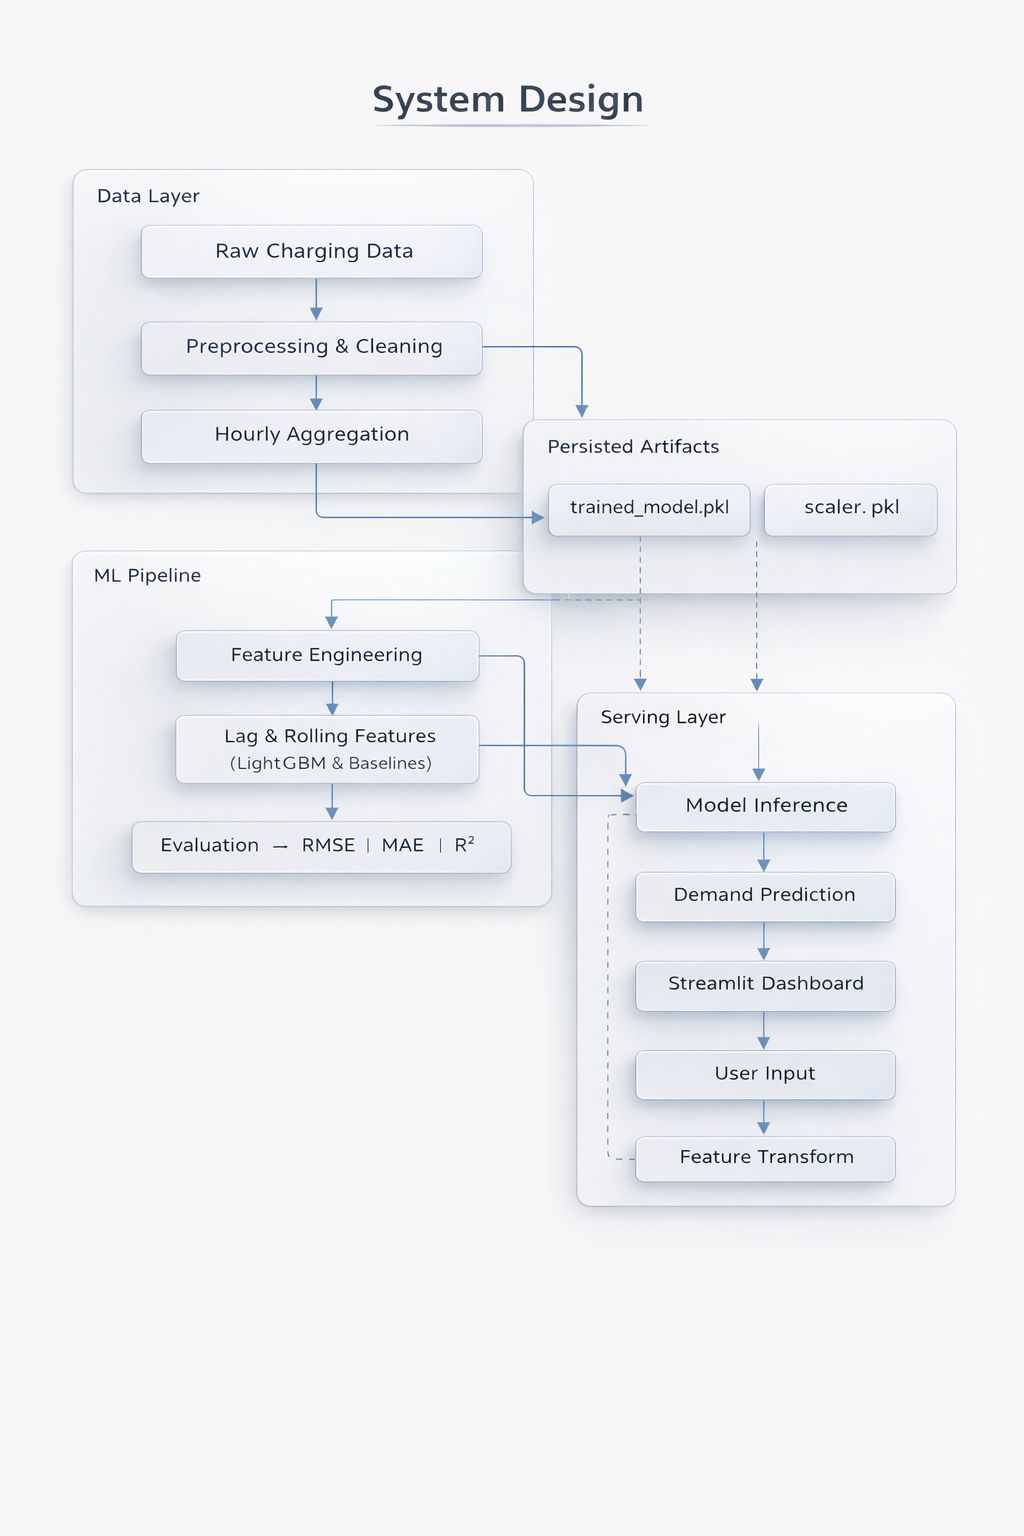
\includegraphics[width=0.5\linewidth]{image1.png}
    \caption{System Architecture}
    \label{Diagram}
\end{figure}
Pipeline Flow:

\begin{enumerate}
    \item JSON Data Ingestion
    \item CSV Conversion
    \item Data Cleaning
    \item Hourly Aggregation
    \item Feature Engineering
    \item Model Training
    \item Model Serialization
    \item Streamlit Deployment
\end{enumerate}

The project follows a modular repository structure:

\begin{itemize}
    \item src/ – preprocessing and training
    \item models/ – serialized models
    \item app/ – user interface
    \item data/ – raw and processed datasets
\end{itemize}
\section{Insights Derived from Data and Model Analysis}

\subsection{Demand Behavior Insights}

Exploratory analysis and aggregated trends revealed the following patterns:

\begin{itemize}
    \item \textbf{Strong Evening Peaks:} Charging demand consistently increases between 17:00–21:00 hours, indicating post-work charging behavior.
    \item \textbf{Weekday Dominance:} Higher average demand observed on weekdays compared to weekends.
    \item \textbf{Station-Level Variability:} Certain stations exhibit significantly higher baseline demand, indicating location-driven usage differences.
    \item \textbf{Right-Skewed Distribution:} Energy delivery per session shows skewness, with occasional high-demand spikes.
\end{itemize}

These patterns confirm that EV charging demand is not random but follows structured temporal cycles.

\subsection{Feature Importance Insights}

Tree-based models (Random Forest / LightGBM) indicated that:

\begin{itemize}
    \item \textbf{Lag Features (lag\_1)} were among the strongest predictors.
    \item \textbf{Rolling 24-hour Mean} significantly improved stability.
    \item \textbf{Hour of Day (cyclical encoding)} strongly influenced predictions.
    \item \textbf{Station Encoded Variable} captured spatial demand differences.
\end{itemize}

This indicates that EV demand has both short-term memory and daily seasonality.

\subsection{Model Performance Insights}

Comparative training revealed:

\begin{itemize}
    \item Linear Regression underperformed, confirming nonlinear demand patterns.
    \item Random Forest improved stability and captured interactions.
    \item Gradient Boosting reduced bias and improved accuracy.
    \item LightGBM demonstrated fastest training and strong generalization.
\end{itemize}

Tree-based ensemble models consistently outperformed the linear baseline, validating the presence of nonlinear feature interactions.
\begin{figure}
    \centering
    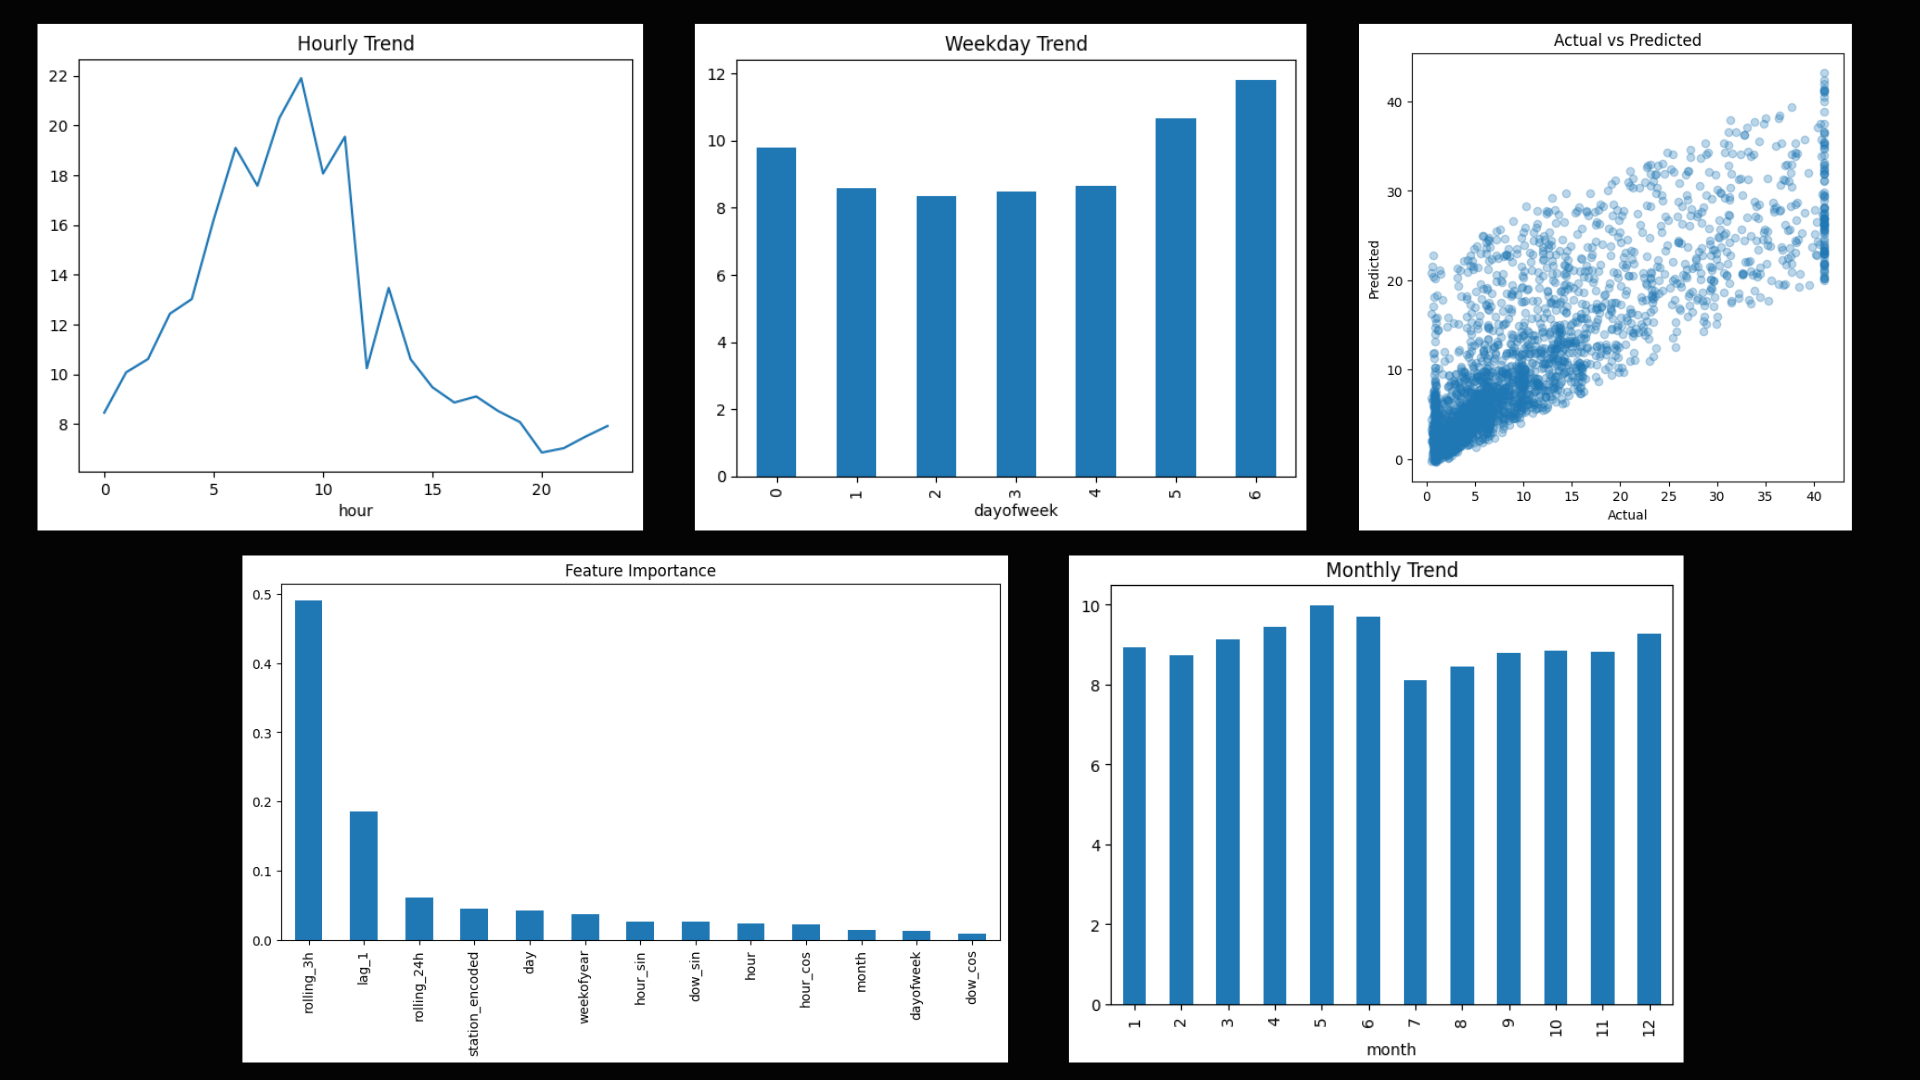
\includegraphics[width=1\linewidth]{image.png}
    \caption{Enter Caption}
    \label{fig:placeholder}
\end{figure}

\subsection{Operational Implications}

The insights suggest:

\begin{itemize}
    \item Peak-hour infrastructure reinforcement is necessary.
    \item Stations with consistently high rolling demand may require additional chargers.
    \item Short-term demand forecasting can help grid load balancing.
    \item Lag-based features allow near-term demand prediction for scheduling optimization.
\end{itemize}

Overall, the model confirms that EV charging demand is temporally structured, location-sensitive, and strongly autocorrelated.

\subsection{Why Accuracy Was Not Used}

Accuracy is not an appropriate metric for this problem because EV demand prediction is a regression task, not a classification task. 
The model predicts continuous numerical values (kWh delivered), rather than discrete class labels.

Accuracy measures the proportion of exact matches between predicted and actual labels, which is meaningful only in classification problems. 
In regression, even a small deviation (e.g., predicting 12.1 instead of 12.4 kWh) would be considered incorrect under an accuracy metric, despite being operationally acceptable.

Therefore, regression-specific evaluation metrics such as MAE, RMSE, and R\textsuperscript{2} were used to quantify prediction error and model performance.

\section{Deployment}

The best model was saved using:

\begin{verbatim}
joblib.dump(best_model, "best_ev_demand_model.pkl")
\end{verbatim}

A Streamlit dashboard was developed for user-friendly demand prediction and visualization.

\section{Optimization}

Performance improvements were achieved through:

\begin{itemize}
    \item Feature engineering
    \item Outlier handling
    \item Ensemble methods
    \item Chronological validation
\end{itemize}

\section{Future Scope}

Future enhancements include:

\begin{itemize}
    \item Hyperparameter tuning
    \item Weather data integration
    \item Real-time streaming
    \item Multi-city deployment
    \item Agentic infrastructure planning (Milestone 2)
\end{itemize}

\section{Conclusion}

This project presents a scalable machine learning framework for EV charging demand prediction. 
Through structured preprocessing, time-series feature engineering, and ensemble modeling, a robust forecasting system was developed. 
The architecture supports future expansion into autonomous infrastructure planning systems.

\end{document}  